\section{A Mente do Robô (Eletrônica e Software)}
\par
\begin{figure}[h]
  \centering
  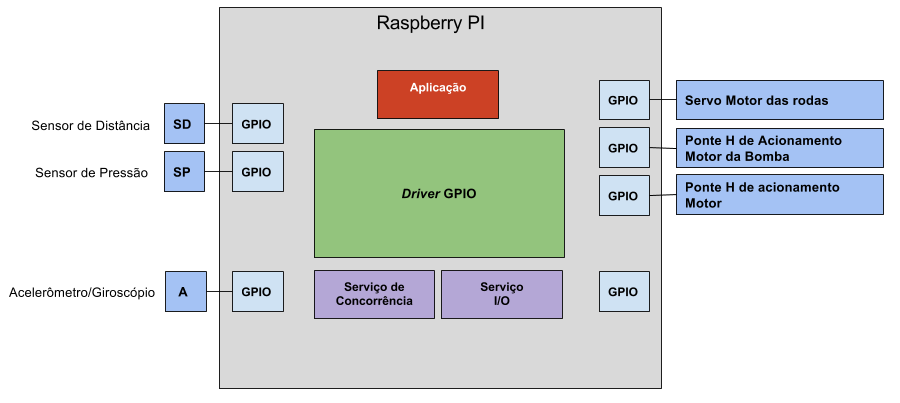
\includegraphics[width=0.8\textwidth]{figures/schema-eletro-soft.png}
  \caption{Interação dos componentes eletrônicos e o core software.}
  \label{fig:schema-eletro-soft}
\end{figure}
\FloatBarrier
\par
Os periféricos fornecerão dados que, por sua vez, serão passados ao driver por meio de dispositivo de \hardware (GPIO). O \textit{driver} será responsável por permitir a comunicação entre o \hardware e o \software que, na Figura \ref{fig:schema-eletro-soft}, é representado pelos Serviços e a Aplicação que deve fornecer ao sistema. Cada serviço tratará os dados de entrada conforme a especificidade solicitada e, em seguida, retorna uma saída para um atuador, por meio do \textit{driver}.

\subsection{Central de Processamentos de Dados}
\subsubsection{Os Requisitos}
Na seleção de uma unidade de processamento o maior fator de seleção foi conseguir uma de forma rápida e com baixo custo, além de ter uma capacidade de processamento suficiente para solucionar os primeiros requisitos vistos da integração entre a área Estrutural (sensores necessários para funcionamento e acionamento de motores e bombas) e a área de \software (capacidade de programar em várias linguagens de programação e uso de \textsf{APIs}), e ter acesso a GPIO. Considerando esses fatos a primeira proposta foi a \rasp, porém por sua limitação de pinos GPIO e a necessidade de muitos pinos para analisar sinais analógicos, foi proposto usar também um arduino, que vem com conversor A/D e já estava disponível para uso. Isso proporcionou a continuidade do trabalho de implementação que já vinha sendo feito sem muitas mudanças devido a alterações trazidas pela área eletrônica.

\subsubsection{Raspberry PI 2 B}
Com o objetivo de desenvolver um robô é necessário ter uma central de processamento de dados. A \rasp  foi escolhida pela sua capacidade de processamento onde pode ser processado as variáveis que fazem o robô tomar decisões na sua rotina. A \rasp aciona a passagem de energia em  relés que fazem o acionamento dos motores que giram as escovas, e do motor da bomba. Como a \rasp não tem conversor A/D foi necesário usar um arduino para tratar o sensor de pressão. A comunicação da \rasp com o Arduino é feito usando protocolo serial  \textsf{UART} (\textit{Universal Asynchronous Receiver/Transmitter}). Também há a possibilidade do uso de várias linguagens de programação e \textsf{APIs}.
\par
\begin{figure}[h]
  \centering
  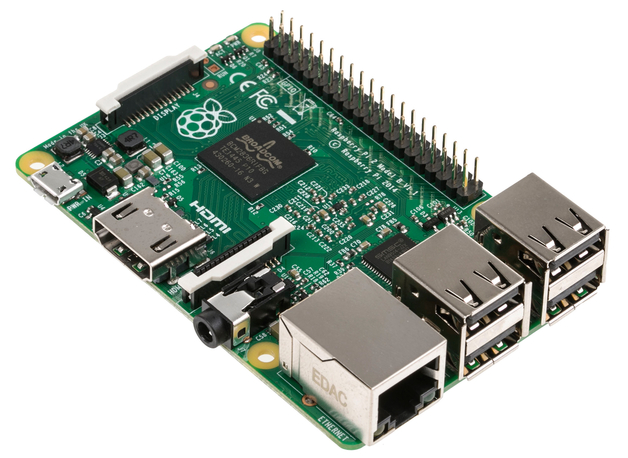
\includegraphics[width=0.6\textwidth]{figures/rpi2b.jpg}
  \caption{Raspberry PI 2 B.}
  \label{fig:schema-eletro-soft}
\end{figure}
\FloatBarrier
\par

\subsubsection{Arduino}
O Arduino Uno foi escolhido a princípio para facilitar o tratamento do sensor de pressão \textsf{MPX-4250}, que possui saída analógica. Trabalhar com conversão A/D na \rasp requer o uso demasiado de pinos (no mínimo 9 pinos para controlar dois sensores, utilizando-se de multiplexadores). Uma vez que o Arduino Uno foi incluido no sistema, delegou-se a ele também o trabalho de controlar os sensores de distância \textsf{HC-SR04}, visto que estes são módulos desenvolvidos para funcionar no arduino.
\par
\begin{figure}[h]
  \centering
  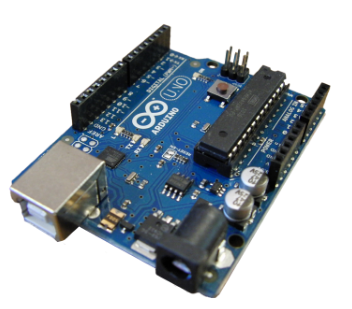
\includegraphics[width=0.5\textwidth]{figures/arduino.png}
  \caption{Arduino.}
  \label{fig:arduino}
\end{figure}
\FloatBarrier
\par

\subsection{O Sistema de Controle de Tensão}
\subsubsection{Os Requisistos/Dimensionamento}
Para acionar os sistemas de alta tensão (Motores e Bomba) com circuitos de baixa tensão (\textit{Raspberry pi}) foram utilizados relés. Com baixas tensões ele induz um campo eletromagnético sobre uma bobina, o que faz com que o relé deixe passar a tensão que está normalmente fechado, caso não haja essa alimentação o relé mantém-se em aberto, efetivamente funcionando como um interruptor.  Como é desejado que em um dos estados o circuito acione o motor e no outro o motor não funcione, foi projetado o circuito electrônico para só acionar o motor em normalmente fechado, em normalmente aberto o motor está em circuito aberto não sendo acionado.
\par
\begin{figure}[h]
  \centering
  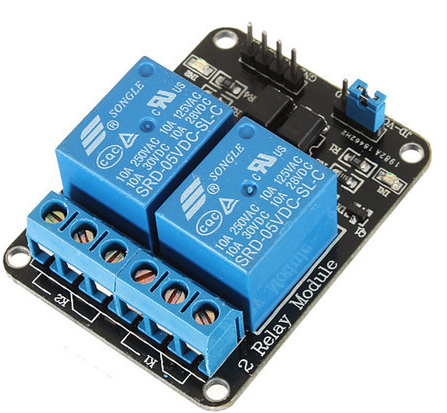
\includegraphics[width=0.4\textwidth]{figures/rele.png}
  \caption{Rele de dois modulos modelo SRD-05VDC-SL-C.}
  \label{fig:rele}
\end{figure}
\FloatBarrier
\par

\subsubsection{GPIO - \textit{Generic Ports Input/Output}}
\textit{Generic Ports Input/Output} são saídas e entradas de tensão. Elas servem para fazer a comunicação do processador com componentes externos, sensores e atuadores e outros tipos de componentes eletrônicos. Algumas dessas portas tem usos predefinidos pelo fabricante do \hardware como saídas de alimentação genérica, e terras, outras dos pinos são de uso genérico. A \rasp tem 40 GPIO, das quais  17 são para uso genérico.
\par
\begin{figure}[h]
  \centering
  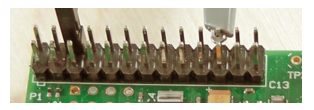
\includegraphics[width=0.6\textwidth]{figures/gpio.png}
  \caption{GPIO Raspberry 1.}
  \label{fig:gpio}
\end{figure}
\FloatBarrier
\par

\subsubsection{\textit{Driver} GPIO}
O \textit{driver} GPIO é um \software que habilita a comunicação entre o \hardware e o \textit{software}. A partir do \textit{driver} é possível receber  os dados advindos dos componentes de \hardware, fazer o devido tratamento e, se necessário, enviar uma resposta ao \hardware (WINDOWS). Para o projeto foram identificadas algumas bibliotecas, disponibilizadas pela comunidade que utiliza o \textit{Raspberry pi}. Essas bibliotecas fazem a interface entre o \hardware e o \textit{middleware}, de forma que essas \textsf{APIs} fazem o papel do \textit{driver}.

\subsection{O Sistema de Sensoriamento}
\subsubsection{Os Requisitos/Dimensionamento}
Para garantir que o robô seja capaz de seguir o percurso definido é necessário que ele seja capaz de detectar as quatro paredes conforme se aproxima de alguma delas. Para tanto, quatro sensores de distância devem ser posicionados em cada uma das laterais do robô. Em caso de colisão com algum obstáculo não detectado pelos sensores de distância e a fim de manter constante o movimento em linha reta do robô, um acelerômetro/giroscópio deve ser utilizado no sistema. Por fim, tanto a pressão interna da caixa de filtragem quanto a externa do robô devem ser medidas constantemente. Caso haja o bloqueio da sucção da bomba por algum detrito haverá também uma variação da pressão interna, que pode ser detectada pelo sensor de pressão e permitir uma resposta imediata do sistema. Para garantir que o robô encontra-se de fato no fundo da piscina conforme ele segue seu percurso, a pressão externa do robô deve ser medida também.

\subsubsection{Os Sensores}
\begin{description}
\item[Sensores de Distância:] serão utilizados sensores de distância com o intuito de permitir ao robô a identificação do espaço entre o robô e qualquer objeto à sua frente. Isso é importante para evitar colisões com as paredes da piscina e obstáculos a alturas que o sensor possa detectar. O sensor de distância ultrasônico \textsf{HC-SR04} foi escolhido  por ser um módulo periférico próprio do arduino, facilitando assim sua implementação. Testes do sensor de baixo d'água ainda precisam ser realizados para validar a escolha.
\item[Sensor de Pressão:] O sensor de pressão proposto funciona com o princípios de materiais piezoelétricos, um liquido entra dentro da câmara e proporciona uma pressão nas paredes da câmara, esse pressão gera uma diferença de potencial no material. Com essa diferença de potencial é possível, usando um conversor A/D (Analógico/Digital), saber a pressão dentro da câmara. Esse sensor sera utilizado para medir a pressão dentro da câmara a onde se encontra a bomba de sucção, assim permitindo que a bomba só trabalhe dentro da pressão ideal de funcionamento, caso algo entupa a entrada da sucção esse sensor detectará  uma queda na pressão interna e por \software o problema sera tratado.
\par
\begin{figure}[h]
  \centering
  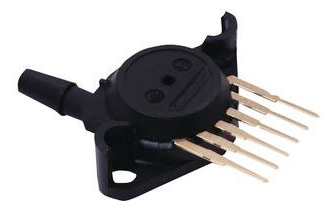
\includegraphics[width=0.4\textwidth]{figures/pressure-sensor.png}
  \caption{Sensor de Pressão}
  \label{fig:a}
\end{figure}
\FloatBarrier
\par
\item[Acelerômetro:] Está sendo cogitado usar um acelerômetro para auxiliar o deslocamento em linha reta do robô e detectar choques com obstáculos grandes, quando ocorre um choque com um obstaculo grande não detectado pelo sensor de distância a uma variação brusca na aceleração, com isso pode-se tratar o obstáculo ou abortar o funcionamento do robô. No mesmo módulo se encontra um giroscópio, ele mede rotações no robô, caso seja identificado alguma rotação não pretendida pelo sistema podemos usar esse dado para corrigir a trajetória. O componente eletrônico que tem os dois sensores comunica-se através do protocolo I2C. Isso reduz o número de pinos necessários pare ler os dados do sensor.
\par
\begin{figure}[h]
  \centering
  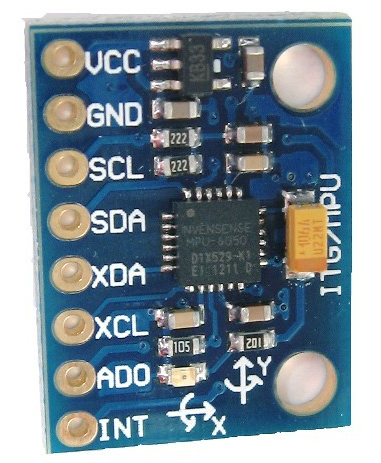
\includegraphics[width=0.3\textwidth]{figures/accelerometer.png}
  \caption{Acelerômetro}
  \label{fig:gpi}
\end{figure}
\FloatBarrier
\par
\end{description}

\subsection{O Sistema de Rotação do Robô}
\subsubsection{Os Requisitos/Dimensionamento}
Foi definido pelo projeto que a propulsão do robô será gerada pela bomba de filtragem. Neste contexto e considerando que o robô move-se idealmente apenas em quatro direcões, existiam duas opções de controle da saída de água da bomba para o controle do direcionamento. A primeira, mais simples, consistia em dispor quatro canos de saída no topo do robô e, por meio de válvulas, controlar quais das saídas seriam abertas de cada vez. A segunda, mais elaborada, consiste em dispor um único cano capaz de rotacionar em 360 graus para se posicionar na direção desejada conforme o robô segue seu percurso. Foi decidido que a segunda opção seria a melhor alternativa, pois ela permite, juntamente com o acelerômetro/giroscópio, corrigir em tempo real qualquer desvio significativo da rota que o robô possa vir a sofrer, além de ser mais barata e de construção mais fácil.

	Conforme o robô segue seu percurso, as rodas devem ser capazes de se manter em duas posicões: horizontal e vertical. Para tanto, um sistema de servos com rotação de 180 graus foi escolhido, similar ao esquema de propulsão.

\subsubsection{Servo Motor}
Servos motores são utilizados para rotacionar um eixo até uma posição desejada. Esses motores são normalmente motores de alto torque. Dois servos (Micro Servo 9g SG90 TowerPro) serão utilizados para rotacionar as rodas, o principal motivo de escolher esse modelo é ele ter torque suficiente para mover as mesmas e ter baixo custo, E para mover a saída de água da bomba foi escolhido um servo motor (SM-S4306R) com maior liberdade de rotação (360º) e uma maior torque.
\begin{figure}[h]
  \centering
	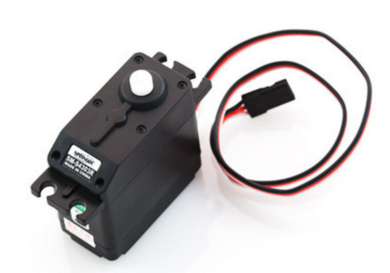
\includegraphics[height=5cm]{figures/servant-motor.png}
	\quad
	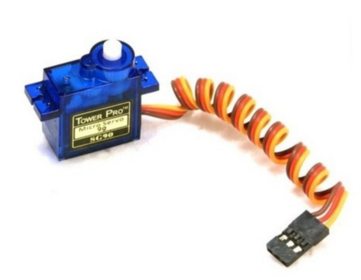
\includegraphics[height=5cm]{figures/micro-motor.png}
  \caption{Servo Motores \cite{flipflop2013} e \cite{flipflop2016}, respectivamente}
\end{figure}
\FloatBarrier

\subsection{Circuito Desenvolvido}
\subsubsection{Diagrama do Circuito}
A Figura \ref{fig:circuit} mostra o diagrama do circuito proposto:
\par
\begin{figure}[h]
  \centering
  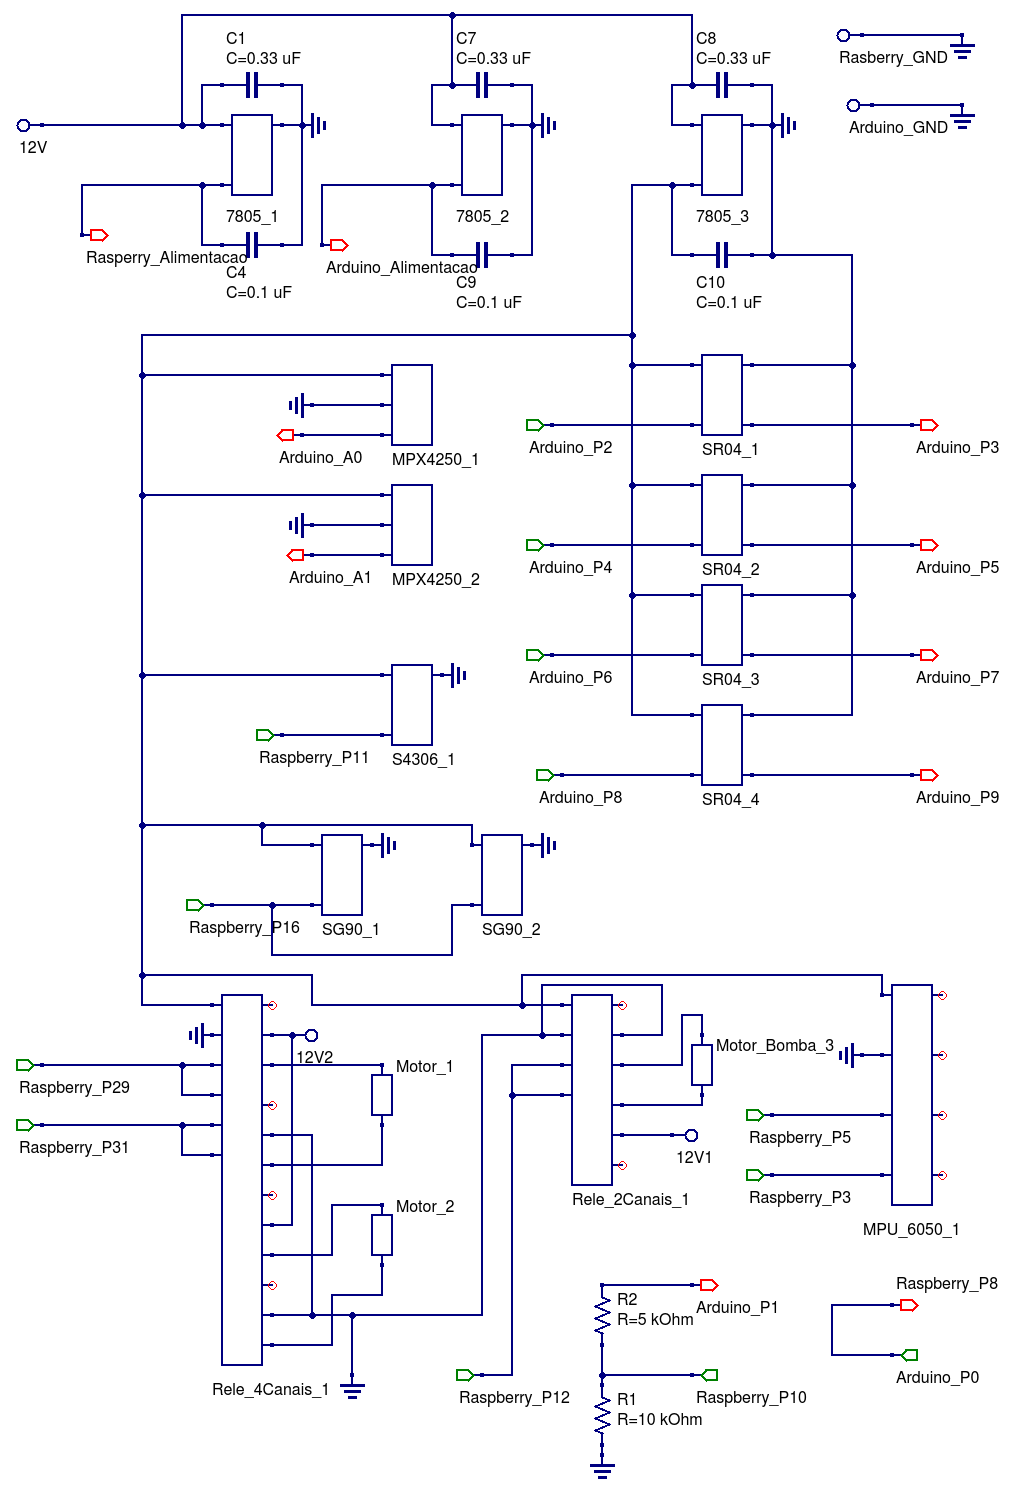
\includegraphics[width=0.8\textwidth]{figures/circuit.png}
  \caption{Circuito proposto.}
  \label{fig:circuit}
\end{figure}
\FloatBarrier
\par

Para a alimentação da \rasp 2 e do Arduino Uno, bem como todos os componentes alimentados em 5V (servo motores, sensores de distância, sensores de pressão), a partir dos 12V oferecidos pela fonte, utilizaram-se reguladores de tensão 7805. Capacitores de 0.33 e 0.1uF foram colocados em paralelo aos reguladores de tensão como medida de segurança.

Conectados a \rasp 2 estão os servo motores SG90 e e S4306, pelos pinos 16 e 11 respectivamente. Para o controle dos motores das escovas e da bomba, utilizaram-se relés para fazer o chaveamento com a tensão de 12V da fonte. O acelerômetro/giroscópio MPU\_6050 é conectado a \rasp via Barramento Serial I2C, para conectar periféricos de baixa velocidade a um sistema embarcado.

A \rasp 2 e o Arduino Uno são conectados por porta serial TX e RX e se comunicam via \textsf{UART}. Um divisor de tensão é usado para conectar o pino TX0 de 5V do Arduino ao pino RXD de 3.3V da \rasp 2.

No Arduino estão conectados os quatro sensores de distância SR04 em portas digitais e os dois sensores de pressão MPX4250 nas portas analógicas A0 e A1.

Até o momento da produção deste relatório, todos os componentes do circuito acima foram testados individualmente, a excessão do acelerômetro e dos relés (ainda a serem obtidos). A montagem do circuito completo em PCB ou placa universal ainda não foi iniciada.

\subsubsection{Pinagem}
A Figura \ref{fig:pinout} mostra a pinagem de cada componente eletrônico do circuito.
\par
\begin{figure}[h]
  \centering
  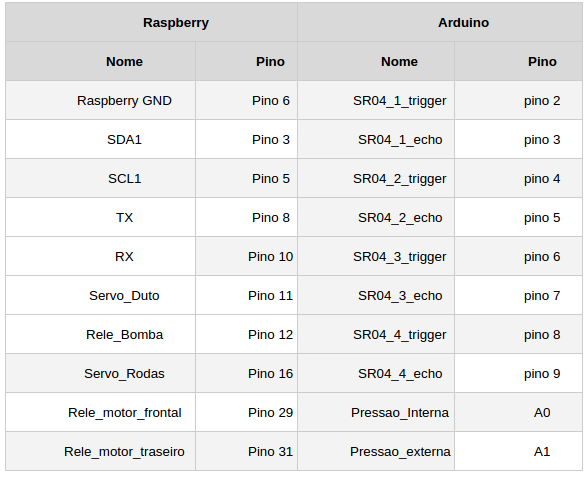
\includegraphics[width=0.8\textwidth]{figures/pinout.png}
  \caption{Pinagem usada.}
  \label{fig:pinout}
\end{figure}
\FloatBarrier
\par

\subsection{Programação e Arquitetura de Software}
A linguagem de programação selecionada inicialmente foi C++ e a biblioteca \textsf{bcm2835.h} para servir como driver de comunicação entre o \software e o \textit{hardware}. No entanto, houve a incompatibilidade entre essa biblioteca e a \rasp 2. A documentação dessa biblioteca (McCauley) diz que ela foi desenhada para funcionar na versão 1 da \textit{Raspberry pi}, mas era compatível com a versão 2, desde que tomadas algumas providências de configuração. Após ter-se feito todo o necessário ainda não estava funcionando corretamente, de forma que a equipe tomou a decisão de mudar de linguagem para \textsf{Python 2.7}, que também possui uma biblioteca de comunicação com a GPIO.

A escolha pela \textsf{bcm2835.h} e C++ foram escolhas em que já se sabia dos riscos e que já foram contornados. Tomada a decisão todo o trabalho já foi convertido para a nova linguagem e vem se mostrando funcional.

A Figura \ref{fig:schema-arch} mostra a abstração da arquitetura do sistema associado ao projeto.
\par
\begin{figure}[h]
  \centering
  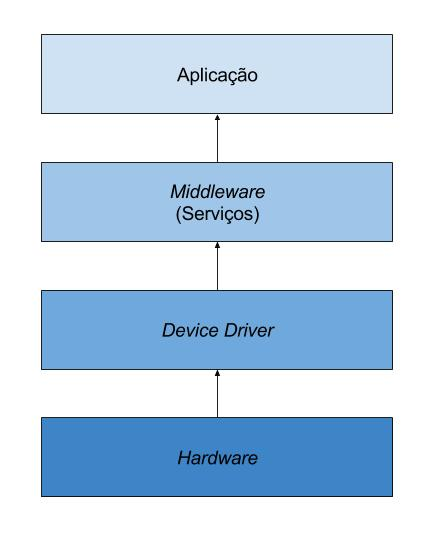
\includegraphics[width=0.5\textwidth]{figures/schema-arch.jpg}
  \caption{Visão geral da arquitetura de software.}
  \label{fig:schema-arch}
\end{figure}
\FloatBarrier
\par

\subsubsection{\textit{Middleware}}
\textit{Middleware} é um \software que conecta outros componentes de \textit{software}. Uma camada de infraestrutura que viabiliza o desenvolvimento de aplicações voltadas ao negócio. Provê serviços que serão amplamente utilizados pela aplicação de negócio (ORACLE). O \middleware fornecerá serviços base para o robô, como ativação dos motores, escova e uso dos sensores.

\subsubsection{Camada de Serviços}
\subsubsubsection{Os Requisitos}
Por meio de reuniões com a equipe de Estruturas a equipe de Lógica identificou algumas ações que o robô precisaria fazer:
\begin{itemize}
\item Identificação de profundidade na piscina.
\item Constante análise da distância entre o robô e obstâculos.
\item Acionamento dos diversos sistemas do robô, como locomoção e filtragem.
\item Comunicação entre os dois componentes do sistema de processamento de dados.
\end{itemize}

A partir desse levantamento e considerando como comumente é definida arquitetura para \software em sistemas embarcados, percebeu-se a necessidade de dois serviços: um serviço para comunicação (entrada/saída de dados) e um para lidar com concorrência de requisições. Assim, a Figura \ref{fig:layer-soft} detalha melhor a comunicação entre as camadas propostas da arquitetura, considerando-se os serviços a serem utilizados e as funcionalidades na camada da aplicação.

\par
\begin{figure}[h]
  \centering
  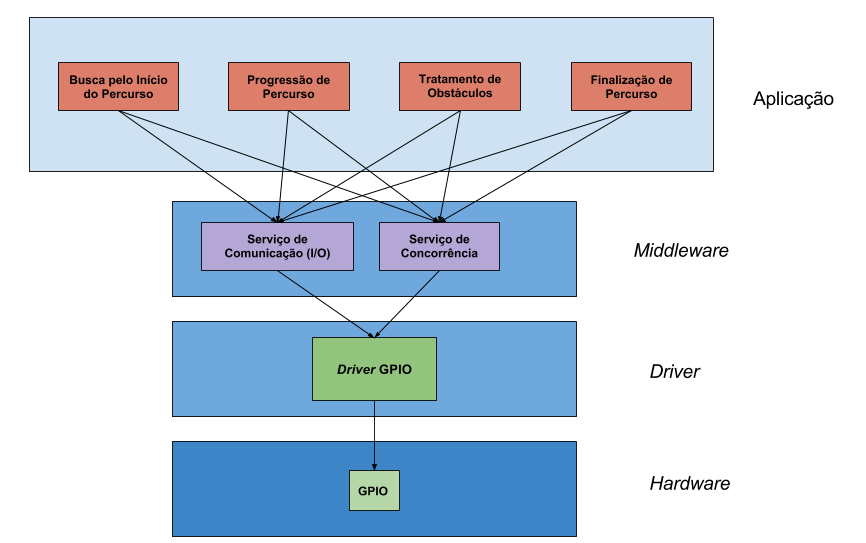
\includegraphics[width=\textwidth]{figures/layers-soft.png}
  \caption{Visão detalhada das camadas de software.}
  \label{fig:layer-soft}
\end{figure}
\FloatBarrier
\par

\subsubsubsection{Serviço de Comunicação (I/O)}
Esse serviço tem por propósito fazer a ponte de comunicação entre o \textit{driver} e a aplicação. Dessa forma, a camada de serviço, por meio do serviço de I/O, deixa invisível para a camada de aplicação como se dá o processo de comunicação com as camadas mais baixas. Isso permite melhor entendimento do código, bem como a possibilidade de refatoração mais simples, na medida em que há um desacoplamento entre as duas partes, comunicação e aplicação. Assim, uma alteração na camada de serviço não terá impacto na camada superior, de serviço, pois a interface entre as duas se manterá. As mudanças internas à camada não interferem no funcionamento de outra.

Abaixo segue a listagem do código até o momento do serviço de comunicação.
\begin{lstlisting}[language=Python, label=services, caption=Código da Camada de Serviços - Serviço de Comunicação]
import pinout as pin
import time
import serial
import RPi.GPIO as GPIO
import time 


pmw_dute = GPIO.PWM(pin.SERVO_PUMP,50)
pmw_dute.start(5) 
def start_arduino():
    arduino_communication = serial.Serial("/dev/ttyAMA0", 115200)
    return arduino_communication


def read_arduino(arduino_communication):
    response = arduino_communication.readline()
    return response     


def write_arduino(arduino_communication, line):
    arduino_communication.write(line)
    return


def activate_pump():
   GPIO.output(pin.WATER_PUMP, GPIO.HIGH)
    return True

def deactive_pump():
    GPIO.output(pin.WATER_PUMP, GPIO.LOW)
    return False


def activate_brush():
    GPIO.output(pin.BRUSH, GPIO.HIGH)
    return True


def deactive_brush():
    GPIO.output(pin.BRUSH, GPIO.LOW)
    return False


def turn_servos_wheels(angle):
    duty = float(angle)/20 + 2.5
    pmw.ChangeDutyCycle(duty)      
    return


def turn_servo_pump(angle, direction):
    time_s = angle/270
    if (direction == 1):
        pmw_dute.ChangeDutyCycle(50)
        time.sleep(time_s)  
    else:
        pmw_dute.ChangeDutyCycle(2.5)   
        time.sleep(time_s)

    pmw_dute.ChangeDutyCycle(100) 
    return
\end{lstlisting}

\subsubsubsection{Serviço de Concorrência}
O serviço de concorrência tem por objetivo abstrair da aplicação questões relacionadas a tarefas que fazem uso do processamento ou de um canal ao mesmo tempo. Isso será comum nas tarefas relativas aos sensores, que devem estar aptos a exercerem suas funções o máximo de tempo possível. Assim, o serviço de concorrência fica responsável por permitir que eles atuem nesses termos, sem que um interfira nas atividades do outro.

\begin{lstlisting}[language=Python, label=services, caption=Código da Camada de Serviços - Serviço de Concorrência]
import thread
import communication as com


semaphore = thread.allocate_lock()

def request_distance(distance, arduino_communication, request_type)
  while True:
    semaphore.acquire()
    com.write_arduino(arduino_communication,request_type)
    distance = com.read_arduino(arduino_communication)
    semaphore.release()
  return distance


def request_pressure(pressure, arduino_communication, request_type)
  while True:
    semaphore.acquire()
    com.write_arduino(arduino_communication,request_type)
    pressure = com.read_arduino(arduino_communication)
    semaphore.release()
  return pressure
\end{lstlisting}

\subsubsection{Camada de Aplicação}
A camada de aplicação da arquitetura fica responsável pelas ações mais alto nível, como locomoção e tomada de decisões. Ela solicita informações para a camada abaixo, a de serviços, e com esses dados faz o tratamento.

Foi escolhida a ação de percorrer o percurso para se trabalhar inicialmente, pois é a que traz mais valor de negócio ao cliente. O robô, após estar na posição inicial numa das quinas da piscina, inicia a sua caminhada até encontrar a próxima parede. Em seguida ele desloca-se para a direita aproximadamente 20 centímetros para então movimentar-se dando “ré”. Ao alcançar a parede faz o deslocamento novamente para a direita de 20 centímetros e repete o processo até encontrar a quina final.

Para essa tarefa o código faz uso dos serviços citados anteriormente e de um conjunto de tomadas de decisões baseadas nos dados recebidos dos serviços. Para demonstrar esse processo foi feito um diagrama de fluxo de dados, apresentado na Figura \ref{fig:move-dfd}.
\par
\begin{figure}[h]
  \centering
  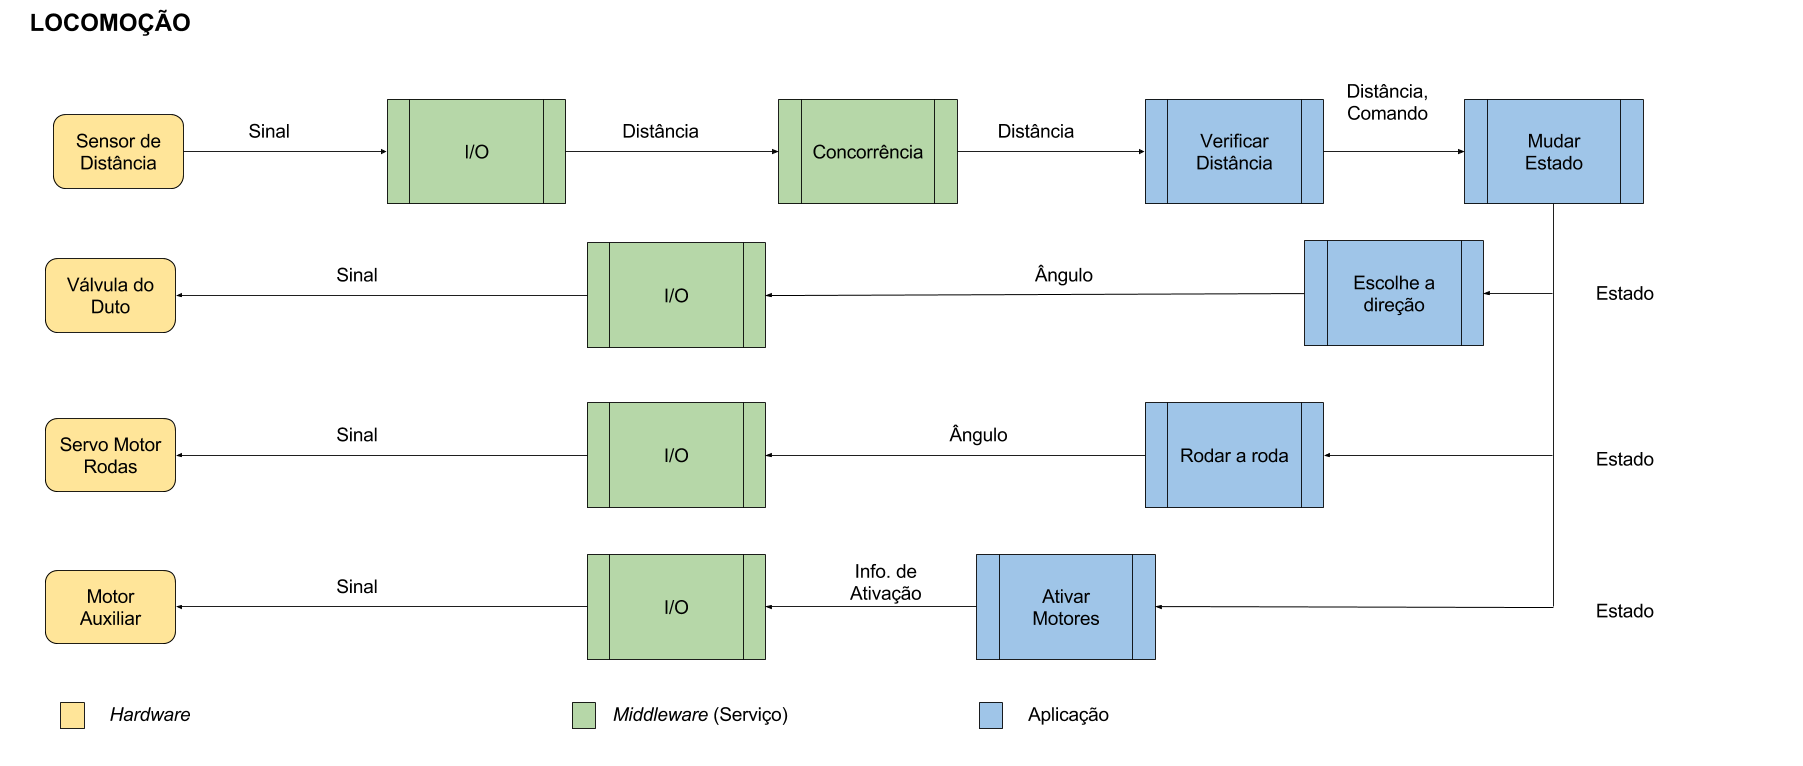
\includegraphics[width=\textwidth]{figures/move-dfd.png}
  \caption{Diagrama de Fluxo de Dados para a Locomoção.}
  \label{fig:move-dfd}
\end{figure}
\FloatBarrier
\par
O código fonte é listado abaixo:

\begin{lstlisting}[language=Python, label=services, caption=Código da Camada de Aplicação]
import time
import communication as SERVICE


FOREVER = True
FRONT = 0
RIGHT = 90
BACK = 180
SIDEWAY = 90
VERTICAL = 0


def find_corner():
    # TODO: Think about the logic of how the CleanPoolRobot will find the
    #       corner of the pool.
    #
    return


def activate_water_pump():
    SERVICE.activate_pump()
    return


def deactivate_water_pump():
    SERVICE.deactive_pump()
    return


def turn_pipe(angle):
    return


def turn_wheels(angle):
    return


def read_front_distance_sensor():
    return 0


def read_back_distance_sensor():
    return 0


def read_right_distance_sensor():
    return 0


def read_left_distance_sensor():
    return 0


def deactivate_brush():
    return 0


def move_front():
    deactivate_water_pump()
    turn_pipe(FRONT)  # degree
    turn_wheels(VERTICAL)  # degree

    activate_water_pump()

    while FOREVER:
        distance = read_front_distance_sensor()  # cm

        if distance <= 5:
            deactivate_water_pump()
            deactivate_brush()
            break

    return


def move_right():
    five_seconds = 5

    deactivate_water_pump()
    turn_pipe(RIGHT)
    turn_wheels(SIDEWAY)

    activate_water_pump()
    time.sleep(five_seconds)  # second

    deactivate_water_pump

    return


def move_back():
    five_centimeters = 5

    deactivate_water_pump()
    turn_pipe(BACK)
    turn_wheels(VERTICAL)

    activate_water_pump()

    while FOREVER:
        distance = read_back_distance_sensor()  # cm

        if distance <= five_centimeters:
            deactivate_water_pump()
            deactivate_brush()
            break

    return


def state_machine(state):
    front = 1
    right = 2
    back = 3

    if state == front:
        move_front()

        previous_state = state
        state = right
    elif state == right:
        move_right()

        if previous_state == front:
            state = back
        else:
            state = front

    elif state == back:
        move_back()

        previous_state = state
        state = right

    return state


def route_course():
    activate_water_pump()

    state = 1

    while FOREVER:
        front_sensor = read_front_distance_sensor()
        back_sensor = read_back_distance_sensor()
        right_sensor = read_right_distance_sensor()
        left_sensor = read_left_distance_sensor()

        if (front_sensor > 5 and right_sensor > 5) or\
           (back_sensor > 5 and left_sensor > 5):
            break

        state = state_machine(state)

    return


def finish():
    # TODO: Think about the logic of how the CleanPoolRobot will turn back
    #       when it finish clean the pool.
    #
    return


def main():
    find_corner()
    route_course()
    finish()

    return

main()
\end{lstlisting}
